% !TeX program = pdfLaTeX
\documentclass[12pt]{article}
\usepackage{amsmath}
\usepackage{graphicx,psfrag,epsf}
\usepackage{enumerate}
\usepackage{natbib}
\usepackage{textcomp}
\usepackage[hyphens]{url} % not crucial - just used below for the URL
\usepackage{hyperref}
\providecommand{\tightlist}{%
  \setlength{\itemsep}{0pt}\setlength{\parskip}{0pt}}

%\pdfminorversion=4
% NOTE: To produce blinded version, replace "0" with "1" below.
\newcommand{\blind}{0}

% DON'T change margins - should be 1 inch all around.
\addtolength{\oddsidemargin}{-.5in}%
\addtolength{\evensidemargin}{-.5in}%
\addtolength{\textwidth}{1in}%
\addtolength{\textheight}{1.3in}%
\addtolength{\topmargin}{-.8in}%

%% load any required packages here



\usepackage{rotating}
\usepackage[table]{xcolor}
\usepackage{tabularx}
\usepackage{makecell}
\usepackage{xcolor}

\begin{document}


\def\spacingset#1{\renewcommand{\baselinestretch}%
{#1}\small\normalsize} \spacingset{1}


%%%%%%%%%%%%%%%%%%%%%%%%%%%%%%%%%%%%%%%%%%%%%%%%%%%%%%%%%%%%%%%%%%%%%%%%%%%%%%

\if0\blind
{
  \title{\bf Inaction on climate change projected to reduce European life expectancy}

  \author{
        Mathew E. Hauer \\
    Department of Sociology, Florida State University\\
     and \\     Alexis R. Santos \\
    Human Development and Family Studies, Pennsylvania State University\\
      }
  \maketitle
} \fi

\if1\blind
{
  \bigskip
  \bigskip
  \bigskip
  \begin{center}
    {\LARGE\bf Inaction on climate change projected to reduce European life expectancy}
  \end{center}
  \medskip
} \fi

\bigskip
\begin{abstract}
Climate change-related excess mortality estimates clearly demonstrate a
dramatic impact on public health and human mortality. However, life
expectancy at birth is more easily communicated and understood by the
public. By properly situating climate change mortality within the
contexts of life expectancy, we better represent the cost of climate
change on longevity. In this paper, we convert excess mortality
estimates due to increases in extreme weather from climate change into
potential reductions in life expectancy at birth in thirty-one European
countries. We project climate change extremes to reduce life expectancy
at birth by 0.24 years for the average European country with differences
in excess of 1.0 years in some countries by the end of the century. We
only estimate the impact of mortality directly related to climate
extremes, making our estimates conservative. Thus, the cost of inaction
on climate change could approach, and likely to exceed, one year of life
in some European countries.
\end{abstract}

\noindent%
{\it Keywords:} climate change, life expectancy, mortality, Europe
\vfill

\newpage
\spacingset{1.45} % DON'T change the spacing!

\hypertarget{main-text}{%
\section{Main Text}\label{main-text}}

Climate change's implications on humanity go far beyond estimates of
economic damages \citep{hsiang2017estimating}, estimates of displacement
\citep{rigaud2018groundswell}, or human conflict
\citep{barnett2007climate} but have the potential to contribute to the
loss of human life \citep{forzieri2017increasing, pachauri2014climate}.
As impact quantification studies move further into the social sciences,
properly quantifying and conveying the impact of climate change on
public health is of increasing importance
\citep{melillo2014climate, cloyd2016engagement}.

Scholars have long estimated the mortality risks associated with climate
change and typically use excess or extra mortality
\citep{forzieri2017increasing, wilson2017climate, mcmichael2006climate, zanobetti2012summer}.
For example, Forzieri et al.~\citeyearpar{forzieri2017increasing}
project climate change extremes to increase European mortality by
150,000+ deaths per year by the end of the century. Although such
estimates are useful, the excess mortality estimates are rather sterile
-- one death is a tragedy, a million deaths a statistic -- and difficult
to relate to on a personal level. Life expectancy at birth (\(e_0\)), on
the other hand, provides potent comparisons of mortality vectors and
converts excess mortality into an intuitively understood metric,
relatable to everyone. To our knowledge, no studies exist that
comprehensively examine the potential reductions of life expectancy due
to climate change. Without properly situating the potential loss of life
within the contexts of metrics such as life expectancy, we risk
underestimating and misreporting the impact of climate change on human
mortality.

Using published data on excess mortality \citep{forzieri2017increasing},
we connect climate change excess mortality to life expectancy in a
mortality model. By estimating the increase in age-specific mortality
rates associated with previously published excess death estimates, we
can assess how much climate change could reduce the anticipated
longevity of the average person in thirty-one European countries. This
approach allows us to quantify the impact of climate change on human
longevity and answer the following question: What is the cost of
inaction on climate change on human longevity? Our results situate
climate change mortality within the broader context of human mortality
and can be used to inform public health interventions and adaptation
measures to prevent such futures.

Our results suggest that climate change could emerge as a potent public
health threat in the 21st century. Mitigation strategies (ie reductions
in greenhouse gas emissions) and adaptation strategies (ie outreach
efforts, retrofitting public buildings, etc.) would help prevent this
new public health concern.

\hypertarget{methods-and-materials}{%
\section{Methods and Materials}\label{methods-and-materials}}

\hypertarget{data}{%
\subsection{Data}\label{data}}

We estimate changes in life expectancy by combining three primary data
sets. First, we use the projected population's by age in conjunction
with projected age-specific mortality rates from the United Nations'
World Population Prospects \citep{united2017world}. This data provides
both the future populations exposed to future climate hazards and the
data necessary to calculate the difference in life expectancy between
baseline, projected mortality and mortality due to climate change.
Second, we use projections of excess mortality due to meteorological
hazards related to climate change from Forzieri et
al.~\citeyearpar{forzieri2017increasing}. This data provides the number
of projected deaths to climate change by the end of the century. And
third, we use cause-of-death distributions from the Global Burden of
Disease study (GBD) \citep{GBD, wang2012age} to distribute Forzieri et
al's \citeyearpar{forzieri2017increasing} projected death totals.

Forzieri et al.~\citeyearpar{forzieri2017increasing} combine data from
the International Disaster Database (EMCAT) and the Natural Catastrophe
Statistics tool (NatCatSERVICE) to create exposure and fatality
statistics related to six weather-related hazards -- heatwaves, cold
waves, droughts, wildfires, river and coastal floods, and windstorms --
and estimate excess mortality associated with those hazards during a
baseline period of 1981-2010 in 28 European countries. They only
considered fatalities \emph{directly attributable} to the event and
\emph{exclude} increased deaths from common causes that were observed to
rise during the event, such as cardiovascular or respiratory
deaths\footnote{``The fatality data from the two databases considered is
  likely to not include increased deaths from common causes that were
  observed to rise at the population level but for which individual
  deaths could not be attributed to the event. For example,\ldots{}
  increased risk of cardiovascular and respiratory deaths \ldots{} may
  be severely under-reported in the EMDAT and NatCatSERVICE.''
  \citep[see][pp.~9, \emph{Supplementary
  Materials}]{forzieri2017increasing}.}. While the disaster data are not
standardized across country, Forzieri et al.~imputed data in incomplete
time periods and countries. This imputation could mask spatial
variability at the sub-national level, but here we use their
country-aggregated results. They downscaled these exposures rates to 1km
grid cells and integrated them into small-area demographic projections
for Europe out to 2100 that correspond to a middle-of-the-road
socioeconomic scenario (SSP2 with medium fertility, medium mortality,
medium migration, and the Global Education Trend education scenario
\citep{jiang2014internal, samir2017human, o2017roads}) and based their
projected mortality on extrapolations of their calculated exposures.
Their results represent business-as-usual climate change and human
development without incorporating potential adaptations to climate
change. They found a potential 150,000+ climate change related
fatalities per year by the mid 2080s with climate change contributing to
90\% of mortality rise as opposed to population changes. The number of
future anticipated deaths are available in their Supplementary Table S8
\citep{forzieri2017increasing} and provide the magnitude of deaths for
our study.

The Forzieri et al.~\citeyearpar{forzieri2017increasing} data contain
only mortality totals and report no age detail, precluding a direct
conversion of excess mortality to life expectancy. To convert excess
mortality to life expectancy, we allocate excess multi-hazard mortality
for each country based on the observed age-specific mortality schedule
for environmental heat and cold exposure deaths from the GBD
\citep{GBD, wang2012age}. Forzieri et al.~found that extreme heat (as
opposed to other five weather-related hazards) account for 99\% of the
anticipated excess mortality by the end of the century. The GBD is the
most comprehensive worldwide data set of epidemiological data and
provides cause-specific mortality by age/sex/geography/year for 249
causes of death in 195 countries and territories. We gather data on
age-specific mortality rates (\(m_x\)) from environmental heat and cold
exposure (cause C.2.9) for the period 2006-2015 for each country in the
study for age groups \(x=0,1,5,10,...95\). These data provide a
mortality schedule to fit the projected climate change excess mortality
from Forzieri et al \citep{forzieri2017increasing}. We assume that the
age-specific mortality schedules observed between 2006 and 2015 due to
environmental heat and cold exposure in the GBD are likely to remain
unchanged in the future. We only use the GBD to distribute the Forzieri
et al.~deaths by age\footnote{GBD data can be retrieved here:
  \url{http://ghdx.healthdata.org/gbd-results-tool?params=gbd-api-2017-permalink/b235b96d60b3b5f06f3e080974c415f3}.}.

With the Forzieri et al data and the GBD we estimate the anticipated
age-specific mortality schedules due to climate change in thirty-one
European countries but we cannot compare life expectancy differentials
in the absence of Climate Change using those two data sets alone. To
create baseline mortality schedules and life expectancy, we gather data
from the United Nations' World Population Prospects (WPP-2017)
\citep{united2017world} for the corresponding European countries in the
period 2080-2085 (the mid-point of the period Forzieri et al.~report
their results \citeyearpar{forzieri2017increasing}). We use the UN
abridged life table data for ages \(x=0,1,5,10,...85\) containing the
necessary mortality rates(\(_nm_x\)), the average number of years lived
in the age-interval (\(_na_x\)), and populations (\(_nP_x\)) for
populations aged \(x\) to \(x+n\).

\hypertarget{methods}{%
\subsection{Methods}\label{methods}}

We derive a number of variables to accomplish our analysis. First, we
use the C.2.9 mortality rates (\(_nm_x\)) from the GBD for ages
\(x=0,1,5,10,...,95\) with the projected populations aged \(x\) to
\(x+n\) from the UN data in the period 2080-2085 (\(_nP_x\)) in country
\(i\) to calculate an un-scaled projection of deaths due to C.2.9
(\(_nD_{x,i}=_nm_{xi}^{GBD} \cdot _nP_x\)). We then abridge \(_nD_{xi}\)
to ages 85+ to match the open-ended age interval found in the UN life
tables. With abridged baseline heat/cold deaths, we proportionally
rescale \(_nD_{x,i}\) to sum to the projected excess mortality for each
scenario \(s\) (\(BASE\), \(LOW\), \(MID\), \(HIGH\)) for each
individual country from Forzieri et al \citep{forzieri2017increasing}
(\(_n\hat{D}_{x,i}\)) and calculate new \(_nm_{xs}^{FORZ}\). \(BASE\)
refers to the baseline mortality rates projected by the UN for the
period 2080-2085 which do not account for climate change. These
calculations combine to create a projected age-specific mortality rates
based on Forzieri et. al's excess mortality.

To calculate life expectancy differentials, we add the age-specific
Forzieri rates \(_nm_{xs}^{FORZ}\) to the projected age-specific
mortality rates found in the published UN life tables \(_nm_x\) to
create a projected \(\hat{m}_x=m_x + m_x^{FORZ}\). We then calculate
life table components \(_nq_x\), \(_nd_x\), \(l_x\), \(L_x\), \(T_x\),
and ultimately \(e_x\) identically for each scenario \(s\) using
standard procedures, substituting \(_nm_x\) with \(_n\hat{m}_x\) where
needed:

\[_nq_{x,i,s} = \frac{_nm_{x,i,s}\cdot  n}{1+(n-_na_{x,i}) \cdot _nm_{x,i,s}}\]
\[_nd_{x,i,s} = _nl_{x,i,s} \cdot _nq_{x,i,s}\]
\[l_{x,i,s} = _nl_{x-1,i,s} - _nd_{x-1,i,s}\]
\[L_{x,i,s} = n \cdot _nl_{x,i,s} + ((n-_na_{x,i,s}) \cdot _nl_{x,i,s})\]
\[T_{x,i,s} = _nL_{x,i,s} + _nT_{x+1,i,s}\]
\[e_{x,i,s} = _nT_{x,i,s} / _nl_{x,i,s}\]

We calculate projected life expectancy reductions due to climate change
related mortality by subtracting \(e_{x,i,s}\) (for scenario \(LOW\),
\(MID\), and \(HIGH\)) from \(e_{x,i,BASE}\) as described by
\citep{beltran2008integrated}.

\hypertarget{reproducible-research}{%
\subsection{Reproducible Research}\label{reproducible-research}}

All data and code necessary to reproduce the reported results are
licensed under the CC-BY-4.0 license and are publicly available in a
replication repository located at
\url{https://osf.io/e43sv/?view_only=f01c29b95a27405b806345e04ced62a8}.

\hypertarget{results}{%
\section{Results}\label{results}}

We find that climate change could alter life expectancy by -0.24 years
(-2.8 months (-0.12 to -0.39 years)) in the average European country
(\textbf{\autoref{figure1}}) by 2100. This reduction is comparable to
mortality due to influenza and pneumonia \citep{arias2013united} in the
United States for the year 2000. Although the average European country
could see a change of -0.24 years, several countries are likely to
experience considerably greater reductions in life expectancy. Spain,
for example, could see a reduction of up to 1.44 years (1.17 - 1.87).

\begin{figure}
\centering
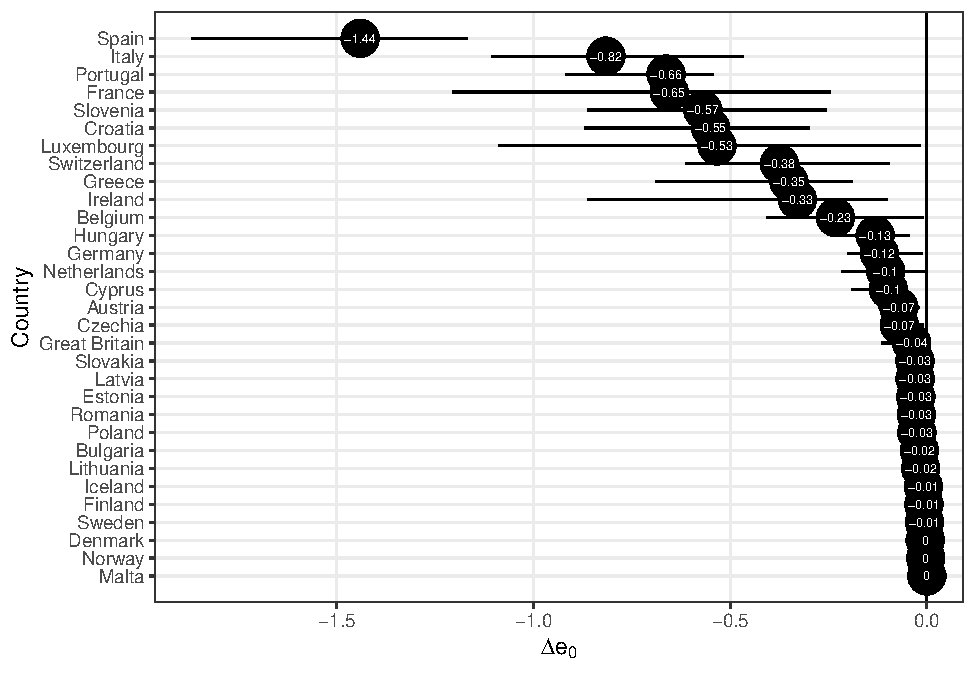
\includegraphics{MANUSCRIPT_files/figure-latex/figure-lollipop-1.pdf}
\caption{Change in life expectancy at birth (\(e_0\)) due to
business-as-usual climate change in the 2080s compared to the projected
\(e_0\). We report changes in life expectancies due to climate change
for thirty-one European countries. The central values represent the
ensemble median while the stems represent the upper and lower bounds of
the inter-model climate variability.\label{figure1}}
\end{figure}

Our results also suggest climate change mortality differentials are
likely to unfold along highly uneven geographies (\autoref{map}).
Whereas many Northern European countries could experience negligible
impacts on life expectancy, seven European countries could see life
expectancy changes in excess of -0.5 years (Spain, Italy, Portugal,
France, Slovenia, Croatia, and Luxembourg). This group of countries
could see life expectancy changes of more than -1.0 years if climate
change hazards are more intense than anticipated. In some countries,
climate change could thus become a bigger killer than trachea, bronchus,
and lung malignant neoplasms (-0.85 years), acute myocardial infarction
(-0.87 years), or all accident related mortality (-0.84 years)
\citep{arias2013united} by the end of the century.

\begin{figure}
\centering
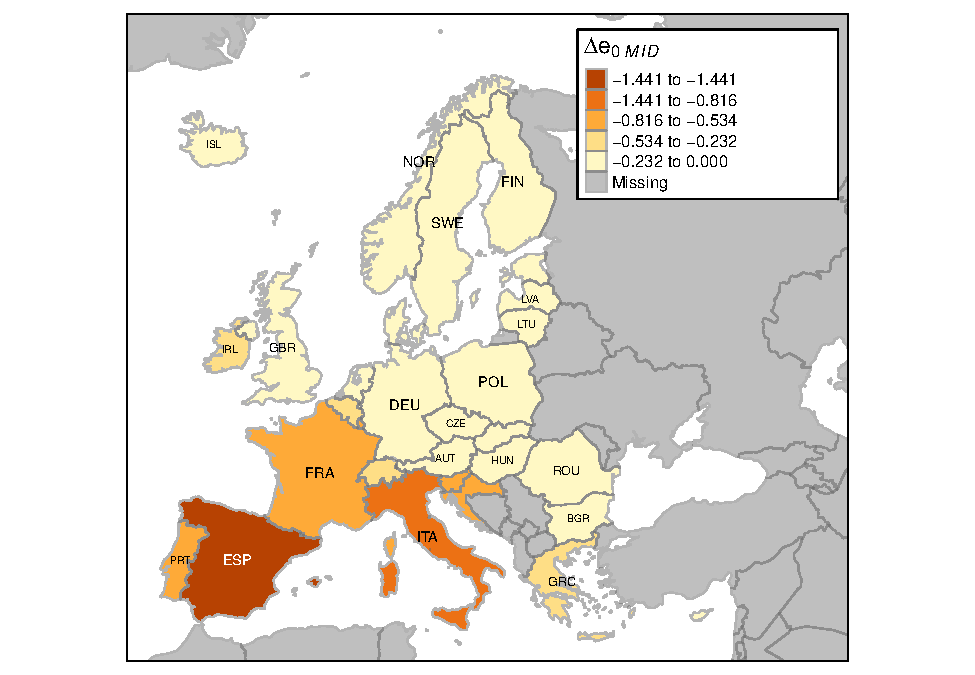
\includegraphics{MANUSCRIPT_files/figure-latex/figure-map-1.pdf}
\caption{Estimated reduction in life expectancy at birth (\(e_0\)) by
the 2080s under the \(MID\) scenario.\label{map}}
\end{figure}

\hypertarget{discussion}{%
\section{Discussion}\label{discussion}}

In this article, we demonstrate the impact climate change could have on
life expectancy at birth due to extreme weather events in thirty-one
European countries. Previous studies on climate change and excess
mortality potentially miscommunicate the impact climate change could
have on human mortality. Contrary to excess mortality estimates, life
expectancy is routinely used as a primary metric for communicating
overall health outcomes and enjoys widespread use by major international
organizations
\citep{world2015world, marmot2012building, salomon2012healthy}. Life
expectancy and its derivatives are the recommended metrics for
population health \citep{parrish2010peer}. Additionally, it connects
mortality estimates into intuitively understandable metrics, translating
global estimates of mortality into personally relatable outcomes. Our
work reveals the extent to which climate change could reduce the average
person's longevity by the end of the century, expanding our
understanding of climate change and public health; thus linking two of
the major areas in current developmental and sustainability discussion
at both national and international levels \citep{abel2016meeting}.

Without adaptation measures, our results suggest climate change could
emerge as a significant new mortality vector and could pose a major
public health threat for some European countries by the end of the
century, echoing previous findings
\citep{forzieri2017increasing, patz2005impact}. Life expectancy has
steadily risen across the world for the last century
\citep{gerland2014world} and our results suggest that climate change
alone could slow these trends in some countries. We expect one European
country to see life expectancy reductions of more than one year under
the middle scenario (Spain), but if climate change has a greater impact
on mortality than anticipated, four European countries (Spain, Italy,
France, Luxembourg) could see life expectancy reductions of more than
one year with Spain experiencing a reduction of nearly two. These
findings highlight the hyperlocalized impacts of climate change
\citep{kendon2014heavier, rosenzweig2010cities, forzieri2017increasing}.

Reductions such as these should not be taken lightly. Many of the
children born today are likely to still be alive by the end of the
century and will be in the age groups (aged 65+) most threatened by the
biggest mortality risk associated with climate change
\citep{keatinge2000heat} -- extreme heat. Climate change could thus be
one of the most aggressive new mortality vectors to emerge over the last
quarter-century, representing a major threat to public health in many
parts of Europe.

Prospective studies on the emerging threat from climate change rely on
linking contemporary mortality with future mortality. However, climate
change could reshape future mortality through other causes of death.
Climate change affects health behaviors that in turn increase mortality
risk through increased alcohol and substance abuse, violent behavior,
insecurity, increase in post-traumatic stress due to weather-related
trauma, increase in stress due to climate change and schizophrenia,
increase in the use of medications that reduce the ability to perspire
and sweat, etc. \citep{patz2005impact} The International Classifications
of Diseases and Related Health Problems (ICD) does not contain ``climate
change" as an official cause of death, so we can only speculate that the
impact of climate change could be larger than reported here. Although we
do not model these potential impacts, our results could thus be
considered conservative.

These results should also be considered conservative when compared to
the broader impact of climate change on human longevity. The disaster
databases that Forzieri et al \citep{forzieri2017increasing} use in
generating their excess mortality estimates probably, though the
disaster databases are unclear, only account for the deaths certified as
\emph{directly} caused by these hazards and are unlikely to capture the
overall numbers associated with these deaths. If the certification of
deaths due to weather extremes is similar to the certification in the
present, than our results and those of Forzieri et al reflect the excess
mortality directly attributable to climatic extremes. Despite this
limitation, the impact of these extremes on \(e_0\) is considerable,
even if conservative.

We also share the concerns of Lee et al.~\citep{lee2017comprehensive}
concerning the business-as-usual climatic assumptions. It is likely that
many countries and communities will deploy a wide variety of adaptation
measures \citep{haines2006climate, kovats2003methods, ebi2006approach}.
These adaptation measures rely on accurate information about the
potential mortality vectors. Our models and those produced by Forzieri
et al.~\citep{forzieri2017increasing} present plausible scenarios on the
potential impact of climate change on human mortality and provide
crucial information to public health officials, national governments,
and international organizations. The time frames associated with climate
change allow ample time for this potential health crisis to be averted.

Finally, we would like to point out that future research should not only
transform excess mortality into life expectancy decrements. Given the
influence of climate change in diseases and causes of death, it is
imperative to quantify the extent to which climate change will derive in
increasing costs for health care systems in these countries. The health
care structures are being taxed by population aging
\citep{rechel2009can} and rising health care costs, yet it remains
unclear how climate change will exacerbate these pressures.

\bibliographystyle{agsm}
\bibliography{ccmort.bib}

\end{document}
